%!TEX root = ../dissertation.tex
% this file is called up by thesis.tex
% content in this file will be fed into the main document

%: ----------------------- introduction file header -----------------------
% the code below specifies where the figures are stored
\graphicspath{{3-mir/figures/}}

\chapter{Music Information Retrieval for Transcription}
\label{ch:mir}

Being able to accurately identify all musical events from audio and transcribe them into musical notations is an essential skill for musicians as well as a paramount goal of music machine learning research.
Enabling an automatic conversion between musical audio and symbolic notations, automatic music transcription opens up many new possibilities.
The most straightforward application of automatic music transcription would be a software tool that transcribes audio recording and produces a musical score, which can aid musicians in various situations.
Automatic music transcription can help build a melody database to be used for music retrieval systems, such as query by humming \cite{molina2014humming}, where it is often very hard to obtain annotated data even when the audio files are abundantly available.
Similarly, by building a database containing symbolic information of music, music recommender systems can leverage the database to infer how much individual users would prefer the music, based on melodic, harmonic, and instrumental information present in the transcription.


As previously stated, due to the complexity and difficulty of creating a completely end-to-end music transcription system, many existing approaches focus on a specific subtask of the problem \cite{casey2008mir}, e.g. extracting onsets and beats, recognizing timbre and instruments, tracking monophonic and polyphonic pitches, or separating audio sources from a mixture.
Each of these subtasks poses interesting goals and applications even without the lofty goal of end-to-end music transcription, and they are often classified under the umbrella term of \emph{music information retrieval} (MIR).
Although this term has existed since 1960s \cite{kassler1966mir}, it was only after the late 1990s when active research on this area has spun off from computer music and computational musicology literature.
During the last two decades, numerous sophisticated and novel approaches for each of these subproblems have been introduced, that have continuously improved the performance in terms of the accuracy in predicting the correct annotations.
This chapter starts by introducing the standard pipeline of music information retrieval that are commonly employed in most MIR models and reviews the state-of-the-art techniques in each area relevant to music transcription.
The purpose of this chapter is not to provide an all-encompassing survey over the history of MIR research but to show a clear common pattern over the areas of MIR where the machine learning models have been evolving from simple heuristics based on hand-crafted features to sophisticated deep learning models with millions of parameters.
Together with the fast progress of the research on deep generative models as shown in the previous chapter, the content of this chapter provides justification and motivation for pursuing research on deep generative models for music transcription, which generally requires more sophisticated statistical models and therefore more powerful hardware than the discriminative counterpart.


\section{The Standard Pipeline}

Audio data is huge in volume; a typical audio track contains 44,100 real-numbered samples per second, and sometimes even more.
Therefore, computational methods for extracting musical information from audio usually contains a pipeline of feature extraction stages to reduce the volume and increase the interpretability of input data, as shown in Figure \ref{fig:pipeline}.
The pipeline includes a few techniques widely used in speech processing, as well as many feature extraction stages created for music-specific purposes.

\begin{figure}[t]
	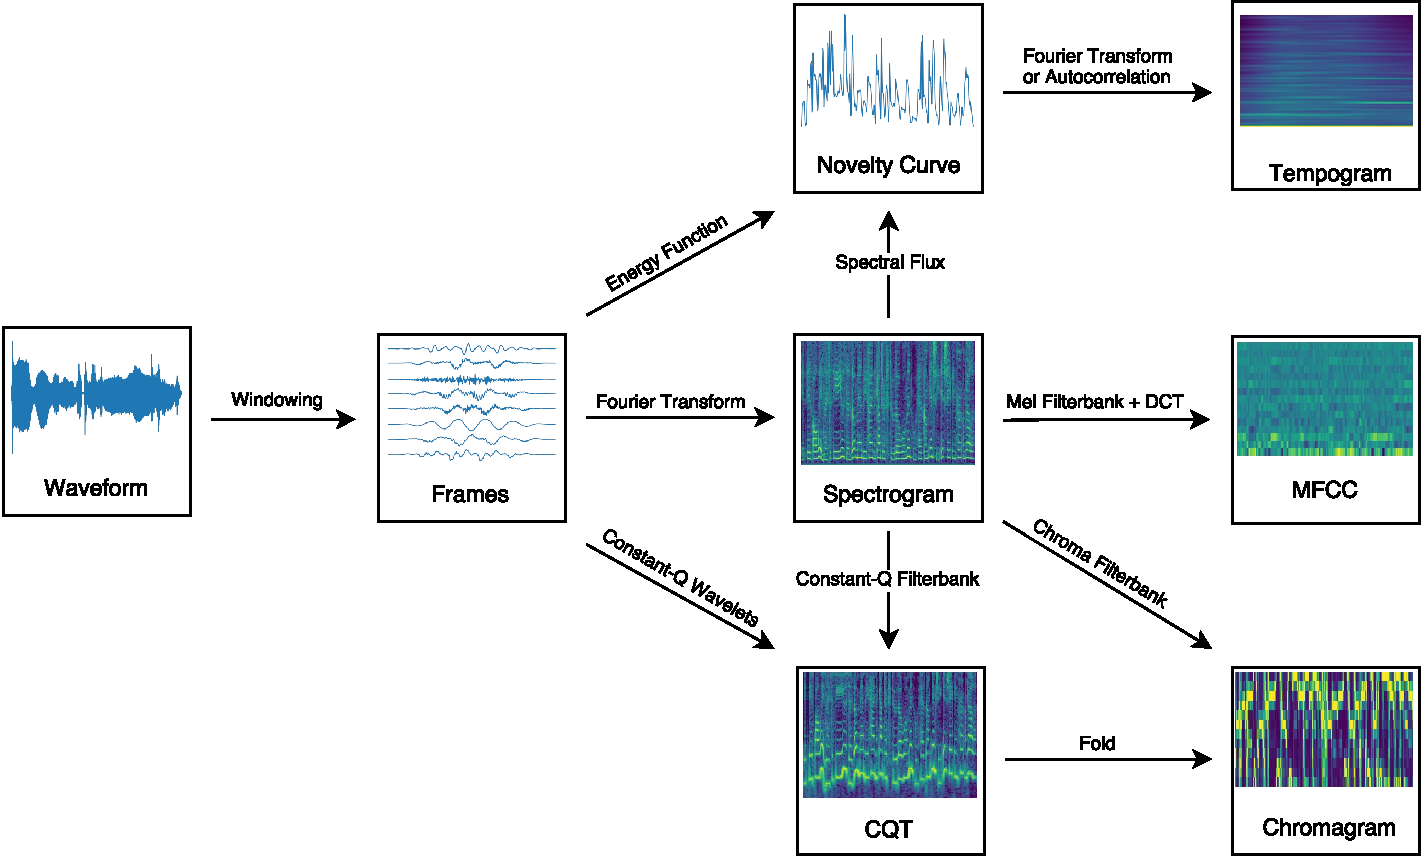
\includegraphics[width=\textwidth]{pipeline.pdf}
	\caption{\small The standard pipeline for music feature extraction. An appropriate set of feature extraction methods needs to be heuristically selected depending on the task.}\label{fig:pipeline}
\end{figure}

While there are many MIR tasks that operate on the track level, such as music recommendation, tagging, and genre classification, most subtasks of music transcription involve the prediction of labels that are dependent on time, operating either in the sample-level or frame-level.
Frames are created by taking a series of overlapping short-time audio segments, where the length of a segment typically ranges from 10 to 50 milliseconds, and optionally multiplying them by a windowing function.
Taking discrete Fourier transforms on the frames produces a \emph{short-time Fourier transform} (STFT), and the magnitude of an STFT gives a \emph{spectrogram}.
Spectrograms give very rich information about the audio; for example, the contour of melodies and the dynamics of music are usually identifiable from the spectrogram image.
Spectrograms are expressive enough to be used as an output of sound synthesis or a source separation algorithm, and the corresponding audio signals can be reconstructed without incurring significant perceptual inconsistencies \cite{griffin1984lim, leroux2010spectrogram}.
However, the dimensionality of a spectrogram is still quite high, making it computationally prohibitive to run many algorithms directly on an STFT or a spectrogram.
This necessitated further transformations by the means of filterbanks, such as \emph{Mel-Frequency Cepstral Coefficients} (MFCC) \cite{logan2000mfcc} by applying the Mel filterbank which is inspired by the human auditory perception.
\emph{Constant-Q transform} (CQT) \cite{schorkhuber2010cqt} uses a filterbank where the center frequencies of filters have a constant Q factor, which is the ratio between the center frequency and the 3 dB bandwidth of a filter.
By configuring CQT to produce 12 filters per octave, it is possible to obtain the coefficients corresponding to each musical tone, and to fold the representation to produce a \emph{chromagram} \cite{bello2005chromagram}.
To extract the beat and tempo information, a heuristic function, such as the first-order difference of the time-domain log energy function or the \emph{spectral flux} that measures the total energy increase over the STFT frequency bins, is applied to formulate a novelty curve, which measures energy bursts typically present in the onsets of notes \cite{bello2005onset}.
The onset information can then be further processed to obtain tempo information via \emph{tempogram} \cite{cemgil2000tempogram} or cyclic tempogram \cite{grosche2010tempogram}.


Once an appropriate set of features are obtained, the next steps for MIR algorithms typically involve applying a classification model.
Examples include Random forests, support vector machines (SVM), and Gaussian mixture model (GMM) classifiers that have been applied to music tagging \cite{ness2009tag}, melody extraction \cite{bittner2015contour}, and genre classification \cite{tzanetakis2002genre} tasks.
Hidden Markov models (HMM) are widely employed for modeling sequence data such as chord progressions \cite{cho2010chord} as well as to smooth the sequence output as a post-processing step \cite{khadkevich2009hmm}, often paired with Gaussian mixture models as the emission probability distribution.
Since finding a better feature representation played a crucial role in earlier MIR systems, many approaches focused on engineering sophisticated feature transformations \cite{harte2006tonnetz} and devising clever pre- and post-processing steps \cite{oudre2009chord}.


More recent approaches have successfully eliminated some or all feature transformation stages in the standard MIR pipeline by training a deep model to learn the feature from the spectrogram or audio waveforms.
Applications of deep learning arose in virtually all types of MIR tasks, including melody extraction \cite{bittner2017deepsalience}, beat tracking \cite{vogl2017drum}, and genre classification \cite{oramas2017genre}.
Apart from a small number of end-to-end approaches, most deep learning models for music still rely on predefined feature transforms such as STFT or CQT, because those features make it easier for a model to learn meaningful concepts without overfitting, using a smaller amount of parameters and thus using less powerful hardware.
In theory, however, any feature extraction stage induces a loss of information, and it suggests that the best-performing model would benefit most from the raw audio data.


\section{Multiple Fundamental Frequency Estimation}

Among the aforementioned subtasks of automatic music transcription, estimating the pitch from polyphonic recording poses the most difficult challenges, as apparent from the recent stream of results from MIREX challenges \cite{downie2014mirex}.
The task is commonly referred to as \emph{multiple fundamental frequency estimation} (Multi-F0 estimation, or MFFE) and is in some sense a superset of the onset and beat detection problems as well as chord and melody tracking problems,
since the frequency tracking task has to indicate the onset and offset of every sound, and tracking chords and melodies becomes much easier when the correct annotations for all pitch contours are available.

Many early methods for MFFE \cite{klapuri2003multiple} focused on extracting features like harmonicity and spectral smoothness from the audio spectrogram and devising a good heuristic for frequency estimation.
Another major technique for polyphonic music transcription is \emph{non-negative matrix factorization} (NMF) \cite{lee2001nmf}, based on the assumption that the spectrogram is a low-rank matrix which is a multiplication of the harmonic profile of each notes and the note activation patterns.
While some approaches \cite{gao2017nmf} based on NMF performs close to the state of the art, it has a drawback of having to obtain duplicate pitch templates for multiple instruments.
Other data-driven approaches are based on dynamic Bayesian networks \cite{raczynski2013dynamic}, hierarchical graphical models \cite{pesek2017hierarchical}, convolutional neural networks \cite{bittner2017deepsalience}, recurrent neural networks \cite{bock2012rnn,sigtia2016endtoend}, and most recently an architecture combining convolutional and bidirectional recurrent neural networks \cite{hawthorne2018piano}.

With the state of the art nearing the perfect accuracies \cite{ewert2017transcription} on the MAPS dataset \cite{emiya2010multipitch} which have been the standard evaluation dataset for piano transcription algorithms, more systematic assessments of transcription models have recently been proposed.
These include the study of invariance under data augmentation \cite{thickstun2017invariances} and the entanglement of note representations that may prevent accurate predictions for unseen combinations of notes \cite{kelz2017entanglement}.

In \cite{li2017infinite}, the idea of using on-the-fly synthesized training dataset for piano transcription was explored, using a simple fully-connected neural network operating on the CQT representation.
The idea of using generative models to predict multiple fundamental frequencies is also not new \cite{dubois2005harmonic,cemgil2006generative}, but they relied on manually designed generative models for sound generation, which might have led to poor generalizability.
Using deep generative models is expected to help overcoming this limitation, since deep learning methods is known to be excellent in learning embeddings and manifolds that are generalizable to different tasks and domains.


\section{Music Synthesis and Translation Models}

While sound synthesis is a topic that has a long history \cite{cook2002synthesis}, recent deep generative have been very successful in synthesizing breathtakingly high-quality audio signals.
We would want the synthesized music and audio signals to capture the long-term dependencies such as beats, measures, and chord progressions that ranges up to a few seconds, while the raw audio signals typically have the order of 10 thousand sameples per second.
This made end-to-end synthesis models more difficult to train than image synthesis and translation models which it usually suffices to capture dependencies ranging a few hundred pixels.
SampleRNN \cite{mehri2016samplernn}, previously discussed in Chapter \ref{ch:deeplearning} in the context of deep autoregressive models, is one of the first successful deep generative models for audio and formed a basis for the techniques used by Lyrebird, an AI startup founded by University of Montr\'{e}al students that provides API for synthesized voice of a specific person, e.g. Barack Obama.
WaveNet \cite{oord2016wavenet}, developed by Google DeepMind, uses a causal architecture using dilated convolutions to generate time-domain audio samples, and is able to produce realistic human voices and piano sounds.
WaveNet learns acoustically meaningful representations including pitch and spectral features \cite{hua2018wavenet}.
There also exist faster approaches using recurrent neural networks to produce vocal and musical audio, as found in \cite{nayebi2015gruv} and \cite{kalingeri2016generation}, albeit with lower quality when compared to WaveNet.
Tacotron \cite{wang2017tacotron, shen2018tacotron} is a fully end-to-end speech synthesizer that works directly on a sequence of characters, which can learn the pronunciation of unseen complex words and different ways of reading the same word according to the phrase semantics and punctuations.
A newer RNN-based model called WaveRNN \cite{kalchbrenner2018wavernn} is capable of generating audio that matches WaveNet in quality, yet with an enough efficiency to be able to run real-time on GPUs or even on mobile phones.
A singing synthesis model \cite{blaauw2017singing} based on the WaveNet architecture is also capable of synthesizing voice parametrically, separating the influence of pitch and timbre in the model.
A music synthesis technique employing a similar approach as the above will be a key component of the overall architecture, allowing the transcription model to generate realistic-sounding music to compare with the input audio.


Audio translation problems concern mapping input audio to a corresponding output with some desired properties, such as speech with reduced noise, singing voice separated from music, or the same speech in the voice of a different speaker.
The \emph{U-Net} architecture \cite{ronneberger2015unet} uses an encoder-decoder framework with skip connections between the hidden layers at the same level of abstraction to perform image translation, and a singing voice separation model can be trained using this architecture \cite{jansson2017separation}.
The encoder-decoder architecture with skip connections can also be trained with GAN objectives, and a few audio translation models working on spectrograms have been developed; examples include singing voice separation \cite{fan2017svsgan, stoller2017separation}, source separation \cite{subakan2017gan}, and speech enhancement \cite{pascual2017segan, donahue2017segan}.

A problem of producing spectrograms as an output of image translation model is that reconstructing the resulting audio requires the phase information.
While using the phases from the input STFT can produce acceptable results for a translation model, a phase reconstruction algorithm is required for a generative model for audio.
A GAN architecture using one-dimensional convolutions called \emph{WaveGAN} was recently introduced \cite{donahue2018wavegan}, which is capable of generating 1-second audio segments from the latent representations.
The 1-D output does not require phase reconstruction, and it was able to achieve a better perceptual quality than the audio reconstructed using 2-D GANs.
As shown in the paper, training of 1-D GANs is much more susceptible to the choice of the GAN objective than the 2-D GANs, and training GAN for longer audio sequences and extending it as a tool for disentanglement of latent semantic information or a conditional audio synthesis framework remains as a challenge.

\section{Symbolic Music Processing and Music Language Models}

Symbolic music processing refers to the techniques for processing music at a symbolic level, such as in the form of sheet music, MIDI signals, or piano roll representations.
Problems in this domain includes optical music recognition \cite{rebelo2012omr}, algorithmic composition \cite{fernandez2013ai}, and computational music theory \cite{hamanaka2013computational}, while the subject most relevant to music transcription research would be \emph{music language models}.
A music language model refers to a statistical model, often being a generative model, that encodes music theoretic knowledge to describe the structural composition and arrangement of musical elements \cite{patel2010musiclanguage}, similarly to how computational linguists build language models to describe the structure of natural languages.
A well-designed music language model can be an important component for a generative model for music, because it can serve as a prior for latent representations and can be combined with conditional synthesis models or software instruments to produce audio.

The first systematic approach of applying a linguistic theory to music was the \emph{generative theory of tonal music} \cite{lerdahl1983gttm}, which was inspired by Noam Chomsky's generative grammar \cite{chomsky1966generative} and was influential in music theory, music psychology, and cognitive musicology.
The history of algorithmic composition techniques is decades-long \cite{fernandez2013ai}, while many are artistic approaches rather than optimization problems to build a generative music language model that best approximates the real world music.
Computational methods for building music language models often include applying statistical natural language processing techniques to music, such as a recurrent neural network to build a music language models \cite{sigtia2014lm}.
The latest approaches to generate realistic sound music sequences in the symbolic domain include an application of variational autoencoder \cite{teng2017generating,tikhonov2017generation}, and a generative adversarial network \cite{yang2017midinet}.

\section{Summary}